\documentclass[12pt,a4paper]{extarticle}
\usepackage[T1,T2A]{fontenc}
\usepackage[utf8]{inputenc}
\usepackage[english,russian]{babel}
\usepackage[top=20mm, bottom=20mm, left=30mm, right=10mm]{geometry}
\usepackage[intlimits]{amsmath, empheq}
\usepackage{amsfonts}
\usepackage{setspace}
\usepackage{listings}
\usepackage{color}
\usepackage{indentfirst}
\usepackage{comment}
\usepackage[section, above, below]{placeins}
\usepackage{caption}
\usepackage{subcaption}
\usepackage{float}

\onehalfspacing
\newcommand{\likeheader}[1]{
	\begin{center}
	\textbf{\MakeUppercase{#1}}
	\end{center}
}
\newcommand{\soeq}[1]{%equals auto numeration
\begin{equation}
	#1
\end{equation}
}
\newcommand{\anonsection}[1]{\section*{#1}\addcontentsline{toc}{section}{#1}}%without numeration in table of contents 
% dot filling, see below
\usepackage{tocloft}
\definecolor{mygreen}{rgb}{0,0.6,0}
%change semicolon to defis in pictures:
\RequirePackage{caption}
\DeclareCaptionLabelSeparator{defffis}{ -- }
\captionsetup{justification=centering, labelsep=defffis}
%change Рис. to Рисунок
\renewcommand{\figurename}{Рисунок}
%code listings
\lstset{%
	basicstyle=\footnotesize,
	showstringspaces=false,
	extendedchars=true,
}
% dotfilling in table of contents
\renewcommand\cftsecleader{\cftdotfill{\cftdotsep}}
\def\capfigure{figure}
\makeatletter
     \renewcommand{\l@section}{\@dottedtocline{1}{0.4cm}{0.4cm}}
     \renewcommand{\thesection}{\arabic{section}}
     \renewcommand{\section}{\@startsection{section}{1}{0.6cm}{-3ex plus -1ex minus -.5ex}{2.2ex plus.2ex}{\bfseries\Large}}
\makeatother
\makeatletter
     \renewcommand{\l@subsection}{\@dottedtocline{2}{0.8cm}{0.8cm}}
     \renewcommand{\thesubsection}{\arabic{section}.\arabic{subsection}}
     \renewcommand{\subsection}{\@startsection{subsection}{2}{0.6cm}{-3.5ex plus -1ex minus -.2ex}{2.3ex plus.2ex}{\bfseries}}
\makeatother

%Piece of Lemeshevsky article :)
\newcommand{\un}[1]{\underline{#1}}
\newcommand{\ov}[1]{\overline{#1}}
\newcommand{\half}{\frac{1}{2}}
\newcommand{\ves}[1]{{#1}^{(\sigma)}}
\newcommand{\vesa}[1]{{#1}^{(\sigma_1,\sigma_2)}}
\newcommand{\Ves}[1]{{#1}^{(\Sigma)}}
\newcommand{\Vesa}[1]{{#1}^{(\Sigma_1,\Sigma_2)}}
\newcommand{\eeq}{\end{equation}}
\newcommand{\econ}{\end{constheorem}}
\newcommand{\lsum}[2]{\sum\limits_{#1}^{#2}}
\newcommand{\lint}[2]{\int\limits_{#1}^{#2}}
\newcommand{\lmax}[1]{\max\limits_{#1}}
\newcommand{\lsup}[1]{\sup\limits_{#1}}
\newcommand{{\proof}}{{\par\sc Доказательство.}\,}
\newcommand{\suff}{$\Longleftarrow$~}
\newcommand{\necess}{$\Longrightarrow$~}
\newcommand{\lAll}{~\rule{6pt}{6pt}}
\newcommand{\All}{\lAll}
\newcommand{\all}{\lAll}
\newcommand{\const}{\rm const}
\newcommand{\diver}{\>\rm div\>}
\newcommand{\grad}{\>\rm grad\>}
\newcommand{\Dtilde}[2]{{#1}^{~^{~^{\!\!\!\!\!\!\!\!\!\!\!\approx}}{#2}}}
\newcommand{\DIntilde}[2]{{#1}^{~^{~^{~^{\!\!\!\!\!\!\!\!\!\!\!\!\!\!\approx}}}{#2}}}
\newcommand{\widecheck}[2]{{#1}^{~^{\!\!\!\!\!\!\!\vee}}{#2}}
\newcommand{\wIncheck}[2]{{#1}^{~^{~^{\!\!\!\!\!\!\!\!\!\!\!\vee}}{#2}}}
\newcommand{\hcirc}[1]{\stackrel{\circ}{#1}}
\newfont{\eusm}{eusm10 at 12pt}  % шрифт рукописный
\newcommand \pA {\mbox{\eusm\symbol{65}}}
\newcommand \pB {\mbox{\eusm\symbol{66}}}
\newcommand \pD {\mbox{\eusm\symbol{68}}}
\newcommand \pP {\mbox{\eusm \symbol{80}}}
\newfont{\ieusm}{eusm9}  % шрифт рукописный индексный
\newcommand \ipA {\mbox{\ieusm\symbol{65}}}
\newcommand \ipB {\mbox{\ieusm\symbol{66}}}
\newcommand \ipD {\mbox{\ieusm\symbol{68}}}
\newcommand \ipP {\mbox{\ieusm\symbol{80}}}
\newcommand{\OOmega}{{\Omega^{~^{~^{\!\!\!\!\!\!\!\!\!\!\circ}}}}}
\newcommand{\EOmega}{{\Omega^{~^{~^{\!\!\!\!\!\!\!\!\!\!1}}}}}
\newcommand{\rO}{{\rm O}\,}
\newcommand{\pdt}[1]{{\frac{\partial #1}{\partial t}}}
\newcommand{\pdx}[1]{{\frac{\partial #1}{\partial x}}}
\newcommand{\pdeta}[1]{{\frac{\partial #1}{\partial\eta}}}
\newcommand{\pdtheta}[1]{{\frac{\partial #1}{\partial\theta}}}
\newcommand{\pds}[1]{{\frac{\partial #1}{\partial s}}}
\newcommand{\pdxx}[1]{{\frac{\partial^2 #1}{\partial x^2}}}
\newcommand{\pdtt}[1]{{\frac{\partial^2 #1}{\partial t^2}}}
\newcommand{\pdss}[1]{{\frac{\partial^2 #1}{\partial s^2}}}
\newcommand{\pdxixi}[1]{{\frac{\partial^2 #1}{\partial \xi^2}}}
\newcommand{\psdx}[2]{{\frac{\partial^{#2} #1}{\partial x^{#2}}}}
\newcommand{\psdt}[2]{{\frac{\partial^{#2} #1}{\partial t^{#2}}}}
\newcommand{\pdxxx}[1]{{\frac{\partial^3 #1}{\partial x^3}}}
\newcommand{\fg}[1]{\stackrel{\wedge}{#1}}
\newcommand{\ks}[1]{\left({#1}\right)}
\newcommand{\fs}[1]{\left\{{#1}\right\}}
\newcommand{\kvs}[1]{\left[{#1}\right]}
\newcommand{\norm}[1]{\|{#1}\|}
\newcommand{\enorm}[2]{\|{#1}\|_{#2}}
\newcommand{\dx}{{\partial\over\partial x}}
\newcommand{\parom}{{\partial \Omega}}

\begin{document}

% Title paper
\begin{titlepage}
	\begin{center}
		\normalsize {\bf МИНИСТЕРСТВО ОБРАЗОВАНИЯ РЕСПУБЛИКИ БЕЛАРУСЬ} \\
		\vspace{0.5cm}
		\normalsize {\bf БЕЛОРУССКИЙ ГОСУДАРСТВЕННЫЙ УНИВЕРСИТЕТ} \\
		\vspace{0.5cm}
		\normalsize {\bf Факультет прикладной математики и информатики} \\
		\vspace{0.5cm}
		\normalsize Кафедра математического моделирования и управления \\
		\vspace{3cm}
        КОМОДЕЙ \\
        Владислав Геннадьевич \\
        \vspace{3cm}
		\normalsize {\bf ЧИСЛЕННОЕ РЕШЕНИЕ ЗАДАЧИ СОПРЯЖЕНИЯ УРАВНЕНИЙ ГИПЕРБОЛИЧЕСКОГО И ПАРАБОЛИЧЕСКОГО ТИПОВ МЕТОДОМ КОНЕЧНЫХ ЭЛЕМЕНТОВ}\\
		\vspace{1cm}
		\normalsize Отчет по преддипломной практике \\
		\vspace{2cm}
        \begin{tabbing}
            MMMMMMMMMMMMMMMMMMMMMMMMMMMMMMM \= MMMMMMM \kill
            \> Руководитель: \\
            \> Лемешевский С.В. \\
            \>  кандидат физ.-мат. наук, 
        \end{tabbing}
        \begin{tabbing}
            MMMMMMMMMMMMMMMMMMMMMMMMM \= MMMMMMM \kill
            <<Допустить к защите>> \>  \\
            с предварительной оценкой \underline{\hspace{0.5cm}} \\
            <<\underline{\hspace{1cm}}>> \underline{\hspace{3.3cm}} 2017 г.
        \end{tabbing}

		\vspace{2cm}

        \large Минск, 2017
	\end{center}
\end{titlepage}

\thispagestyle{empty}
\begin{center}
    \normalsize {\bf БЕЛОРУССКИЙ ГОСУДАРСТВЕННЫЙ УНИВЕРСИТЕТ} \\
    \normalsize { Факультет прикладной математики и информатики} \\
    \normalsize Кафедра математического моделирования и управления \\
\end{center}

\vspace{0.7cm}
																								
Утверждаю 


Заведующий кафедрой

\underline{\hspace{3cm}} В.И. Белько

<<\underline{\hspace{1cm}}>> \underline{\hspace{3.3cm}} 2017 г.


\begin{center}
    \bf ЗАДАНИЕ НА ДИПЛОМНУЮ РАБОТУ
\end{center}

Обучающемуся студенту Комодею В.Г.

\begin{enumerate}
	\item Тема работы: Численное решение задачи сопряжения уравнений гиперболического и параболического типов методом конечных элементов

    \item Утверждена приказом ректора БГУ от \underline{\hspace{4cm}} № \underline{\hspace{1cm}}

	\item Исходные данные к работе
		\begin{itemize}
			\item Теория метода конечных элементов.
			\item Размещенные в интернете методические материалы.
			\item Технические требования к электронным версиям отчетных документов.
		\end{itemize}

	\item Перечень графического материала
		\begin{itemize}
			\item Логотип БГУ для включения на слайды презентации.
			\item Графики иллюстраций.
			\item Иллюстрации сравнительного анализа точного и приближенного вычислений.
		\end{itemize}

	\item Перечень вопросов подлежащих разработке или краткое содержание работы
		\begin{itemize}
			\item Рассмотреть постановку задачи.
			\item Разработать приложение для решения .
			\item Графически проиллюстрировать процесс решения.
		\end{itemize}
	\item Дата выдачи задания \underline{\hspace{3cm}}  2017 г.
\end{enumerate}
\textbf{Руководитель работы} \underline{\hspace{6cm}}С.В.Лемешевский
\begin{center}
	(Подпись, дата)
\end{center}
\textbf{Задание принял к исполнению}\underline{\hspace{6.5cm}} Комодей В.Г.
\begin{center}
	(Подпись, дата)
\end{center}
\thispagestyle{empty}
\newpage

\newpage
%align table of contents name 
\renewcommand{\contentsname}{\hfill\bfseries\large ОГЛАВЛЕНИЕ\hfill}   
\renewcommand{\cftaftertoctitle}{\hfill}
\tableofcontents
\newpage

\likeheader{реферат}
\pagestyle{plain}
Дипломная работа, 23 стр., 9 рис., 2 источника, 1 приложение

\textbf{Ключевые слова}: ДИФФЕРЕНЦИАЛЬНОЕ УРАВНЕНИЕ, ВАРИАЦИОННАЯ ПОСТАНОВКА, 
КОНЕЧНЫЕ ЭЛЕМЕНТЫ, FENICS, PYTHON.

\textbf{Объект исследования} --- задача сопряжения уравнений гиперболического и параболического типов.

\textbf{Цель работы} --- численное решение задачи сопряжения уравнений гиперболического и параболического типов

\textbf{Методы исследования} --- метод конечных элементов.

\textbf{Результатами} являются: вычислительный алгоритм и программа решениия задачи сопряжения
уравнений гиперболического и параболического типов

\textbf{Область применения} --- приближенное решение дифференциальных уравнений, математическое
моделирование процессов, протекающих в разнородных средах.

\likeheader{рэферат}

Дыпломная работа 23 с., 9 мал., 2 крынiцы, 1 дадатак.

\textbf{Ключавыя словы} ДЫФЕРЕНЦЫАЛЬНАЕ РАУНАННЕ, ВАРЫЯЦЫЕННАЯ ПАСТАНОУКА, КАНЧАТКОВЫЯ ЭЛЕМЕНТЫ,
FENICS, PYTHON.

\textbf{Аб'ект даследавання} --- задача аб спалучэннi гiпербалiчнага i парабалiчнага раунання.

\textbf{Мэта работы} --- вылiковае рашэнне задачы аб спалучэннi гiпербалiчнага i парабалiчнага раунання.

\textbf{Метады даследавання} --- метад канчатковых элементау.

\textbf{Вынiкамi} з'яуляюцца: вылiковы алгарытм i праграма рашэння задачы аб спалучэннi гiпербалiчнага i парабалiчнага раунання.

\textbf{Вобласць прымяненя} --- прыблiзнае рашэнне дыференцыяльных раунанняу, матэматычнае
мадэляванне працэсау якiя праходзяць у разнастайных срэдах.
\likeheader{summary}

Graduate work. 23 p., 9 pic., 2 sources, 1 appendix

\textbf{Key words}: DIFFERENCIAL EQUATION, VARIATION SETTING, FINITE ELEMENTS, FENICS, PYTHON.

\textbf{Research object}: problem about hiperbolic and parabolic equation conjugation.

\textbf{Work goal}: numerical solution for problem about hiperbolic and parabolic equation conjugation.

\textbf{Research methods} --- finite elements method.

\textbf{Results} --- computational algorithm and program for solving problem about hiperbolic
and parabolic equation conjugation.

\textbf{Use area} --- solution of difference equations, mathematic process work modeling.


\begin{center}
    \anonsection{ВВЕДЕНИЕ}
\end{center}

Задачи сопряжения двух или более дифференциальных уравнений, заданных в различных областях
пространства и связанных на границе раздела некоторыми условиями сопряжения,
возникают при изучении многих реальных задач. Последние возникают при изучении явлений в средах 
с резко отличающимися физическими свойствами. Так, например, к решению задач 
о сопряжении однотипных уравнений второго порядка параболического и гиперболического типов приходят
при изучении стационарных и нестационарных колебательных процессов в областях
составленных из разнородных кусков.

В теории распространения электромагнитного поля, в явлениях магнитной
гидродинамики приводит к задачам сопряжения разнотипных уравнений. В этом случае тип уравнения
определяется свойствами среды и характером процесса. Особое внимание при
этом уделяется условиям сопряжения на границах подобластей. Вопросы
однозначной разрешимости краевых задач для уравнений смешанного типа активно рассматриваются в литературе.

\newpage









\section{Постановка задачи сопряжения для уравнения \\ гиперболо-параболического типа}
Пусть ограниченная область $\Omega \subset  \mathbb{R}^2 $ с границей $\partial \Omega$ разбивается кривой 
$\Gamma$ на две подобласти $\Omega_1$ и $\Omega_2$. В области $\Omega_2$ будем рассматривать уравнение параболического типа,
 а в $\Omega_1$ -- уравнение гиперболического типа по $t$. На $\partial \Omega$ задаются граничные условия, на $\Gamma$ -- условия сопряжения. Задача формулируется следующим образом, для неизвестной функции $u$:
$$
u(x) =
  \begin{cases}
    u_1, \quad x \in \Omega_1\\
    u_2, \quad x \in \Omega_2 \\
  \end{cases}
$$
рассмотрим следующие уравнения:
\begin{equation}
    \pdtt{u_1} = div(k_1(x)gradu_1) + f_1(x, t), \quad x \in \Omega_1,~t > 0,
    \label{eq:def1}
\end{equation}

\begin{equation}
    \pdt{u_2} = div(k_2gradu_2) + f_2(x, t)
    \label{eq:def2}
\end{equation}

Уравнения (1) и (2) дополним граничными условиями Дирихле:
\begin{equation}
     u = 0, \quad x \in \parom.
    \label{eq:dirichlet}
\end{equation}

На границе раздела задаются условия сопряжения:
\begin{equation}
    (k_1(x)gradu_1, \ov n) = (k_2(x)gradu_2, \ov n), \quad x \in \Gamma ,
    \label{eq:conjugation}
\end{equation}
$$ u_1(x,t) = u_2(x, t), \quad x \in \Gamma$$

Также в области $\Omega_1$ задаются начальные условия:
\begin{equation}
     u_1(x, 0) = \varphi_1(x), \quad x \in \Omega_1 
     \label{eq:start1}
\end{equation}

\begin{equation}
     \pdt{u_1}(x, 0) = \psi(x), \quad x \in \Omega_1 
     \label{eq:start2}
\end{equation}

\begin{equation}
     u_2(x, 0) = \varphi_2(x), \quad x \in \Omega_2
     \label{eq:start3}
\end{equation}

Пусть $k(x)$:
$$
k(x) =
  \begin{cases}
    k_1, \quad x \in \Omega_1\\
    k_2, \quad x \in \Omega_2 \\
  \end{cases}
$$

Известно, что задача (\ref{eq:def1}) -  (\ref{eq:start3}) имеет единственное решение 


\section{Метод конечных элементов}
\subsection{Введение в метод конечных элементов}

Метод конечных элементов(МКЭ) — это численная процедура решения задач,
сформулированных в виде дифференциального уравнения или вариационного 
принципа.[2]
МКЭ возник как универсальный метод для решения дифференциальных уравнений. 
Метод приобрел большую популярность, так как он позволяет анализировать и
решать широкий спектр задач.


Метод конечных элементов отличается от классических
методов Ритца и Галеркина тем, что аппроксимирующая функция является
линейной комбинацией непрерывных кусочно-гладких финитных функций.
Финитные функции отличны от нуля только в заданном интервале.
В МКЭ под такими интервалами подразумеваются конечные элементы, на
которые разбивается область $\Omega$. 

Процесс конечно-элементного анализа включает
определенную последовательность шагов. Перечислим эти шаги. 

1. Дискретизация области: построение сетки, задание свойств (материала)
элементов. Область, на которой решается задача, аппроксимируется
(покрывается) непересекающимися подобластями простого типа, которые
называются конечными элементами (КЭ)(Рисунок 1).

\renewcommand{\figurename}{Рисунок}
\begin{figure}[H]
      \centering
      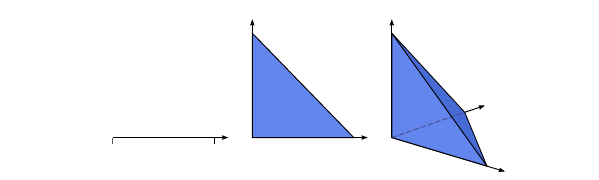
\includegraphics[width=0.8\textwidth]{pics/random-cells.png}\\
      \centering\caption{Пример конечно-элементных подобластей для пространств размерности n = 1,2,3}
\end{figure}
Множество элементов, на которые разбита область, называется конечно-элементной сеткой. Вершины КЭ
называются узлами. Узлы предназначены для описания геометрии элемента
и для задания компонент решения (неизвестная величина задается в узлах).
Компоненты решения в узле называются степенями
свободы. В зависимости от рассматриваемых задач число степеней свободы
в узле различно. Например, если рассматривается задача теплопроводности,
в каждой точке ищется одно значение температуры — одна степень
свободы. А если рассматривается двумерная задача упругости относитель
но неизвестных перемещений, то число компонент будет равно двум, так
как перемещение величина векторная $u = (ux, uy)$. В качестве степеней
свободы могут фигурировать как узловые значения неизвестной функции,
так и ее производные по пространственным координатам в узлах. Кроме 
того необходимо задать свойства материала, из которого изготовлена
конструкция или КЭ.

Как только область разбита на соответствующие подобласти, на каждой такой подобласти можно 
определить функциональное пространство $V$ и использовать каждое $V$ для определения глобального
функционального пространства $V_h$. Подобласть $T$ вместе с определенным на ней функциональным пространством $V$
называется конечным элементом. Более строгое определение:

\begin{itemize}
    \item Подобласть $T$ - замкнута, с кусочно-гладкой границей
    \item Область $V(T)$ - конечное функциональное пространство на $T$
\end{itemize}

2. Выбор аппроксимирующих (базисных) функций. Чаще всего базисные 
функции выбираются в виде полиномов. Поэтому пространство, на котором
ищется решение, является пространством кусочно-полиномиальных
функций. Базисные функции могут иметь различный порядок: линейный,
квадратичный, кубичный и т.д. 

3. Формирование СЛАУ с учетом вкладов от элементов и узлов, введение 
граничных условий в систему уравнений. 

4. Решение полученной системы уравнений.
Точное решение дифференциального уравнения при подстановке в это
дифференциальное уравнение обращает его в тождество в каждой точке.
Решение МКЭ предполагает, что приближенное решение $u_h$ будет удовлетворять
дифференциальному уравнению в узлах сетки $u_h(x_i, t) = u(x_i, t) = u_i^t$.




\subsection{Вариационная формулировка задачи сопряжения \\ гиперболо-параболического уравнения}
Для применения метода конечных элементов к задаче (1)-(6) введем дополнительные пространства:
\begin{equation}
     V = \{u: u_1: x \in \Omega_1; u_2: x \in \Omega_2; u=0, x \in \parom; \text{выполняются условия сопряжения} (4) \} 
     \label{eq:v-space}
\end{equation}

\begin{equation}
     \hat{V} = \{v \in H^1(\Omega), v=0, x \in \parom \} 
     \label{eq:v-hat-space}
\end{equation}


Пространство $H^1$ - пространство Соболева, содержащие такие функции $v$,
что функции $v^2$  и $||\nabla v||^2$ имеют конечные интегралы по области $\Omega$ \\

Вариационная задача строится следующим образом: домножаем уравнения (\ref{eq:def1})-(\ref{eq:def2}) на $v \in V$ с обеих сторон
и интегрируем их по пространству. Уравнение (1) интегрируем по пространству
$\Omega_1$, уравнение (2) интегрируем по пространству $\Omega_2$. \\
Для преобразования подыинтегральных выражений вида $ div(\ov a) v$ применяем формулу Остроградского:

$$ div(\ov a) v = div(\ov a v) - (\ov a, gradv)$$

$$ \int_{\Omega_1} \pdtt{u} v dx  = \int_{\Gamma} v(k_1 gradu_1, \ov n) dS - \int_{\Omega_1}(k_1 gradu_1, gradv)dx + \int_{\Omega_1} f_1vdx  $$

Применим начальное условие Дирихле (3) и получим:

\begin{equation}
    \int_{\Omega_1} \pdtt{u} v dx  = \int_\Gamma v(k_1 gradu_1, \ov n) dS - \int_{\Omega_1}(k_1 gradu_1, gradv)dx + \int_{\Omega_1} f_1vdx 
    \label{eq:1-v}
\end{equation}


$\ov n$ - внешняя нормаль к области $\Omega_1$ от границы $\Gamma$.
Члены вида $(grad u, \ov n)$ - производные по направлению от границы. 
Функция $v$ в литературе называется тестовой функцией(Test Function)[3], $u$ - триальной функцией(Trial Function).

Домножим уравнение (2) на тестовую функцию $v$ с обеих сторон, проинтегрируем полученное равенство по области $\Omega_2$ и применим условие, что $v = 0, x \in \parom$ :

\begin{equation}
    \int_{\Omega_2} v\pdt{u_2} = \int_{\parom_2} k_2(x)v(grad u_2, \ov n)dS - \int_{\Omega_2}(k_2(x) gradu_2, grad v) dx + \int_{\Omega_2} f_2vdx
    \label{eq:2-v}
\end{equation}


К уравнению (\ref{eq:1-v}) прибавим (\ref{eq:2-v}), применяя условие сопряжения (\ref{eq:conjugation}):

\begin{equation}
    \int_{\Omega_1} \pdtt{u_1} v dx + \int_{\Omega_2}\pdt{u_2}vdx  = -\int_{\Omega} k(x)(gradu, gradv)dx + \int_{\Omega} fv dx
    \label{eq:generic}
\end{equation}


Таким образом, мы получили уравнение (\ref{eq:generic}) для всей области $\Omega$ вместо
исходных (\ref{eq:def1}), (\ref{eq:def2}) для $\Omega_1$ и $\Omega_2$. Заметим, что (\ref{eq:generic}) равносильно уравнениям (\ref{eq:def1})-(\ref{eq:def2}).\\

Произведем дискретизацию по времени. Разобьем отрезок $[0, T]$ на $N$ частей с шагом $\tau$
и распишем член $\pdtt{u}$ и $\pdt{u}$ по формуле разностной производной:
\begin{equation}
     \pdt{u} = \frac{u^{n+1}u^{n}}{\tau} 
     \label{eq:pdt-discr}
\end{equation}
\begin{equation}
     \pdtt{u} = \frac{u^{n+1} - 2 u^n + u^{n-1}}{\tau^2} 
     \label{eq:pdtt-discr}
\end{equation}

Домножим на $v$ и проинтегрируем начальные условия (\ref{eq:start2}). Получим:
\begin{equation}
    \int_{\Omega_1}\pdt{u_1}vdx = \int_{\Omega_1}\psi vdx
    \label{eq:psi-v}
\end{equation}

Подставим в (\ref{eq:psi-v}) выражение (\ref{eq:pdt-discr}):
$$\int_{\Omega_1} \frac{u_1^1-u_1^0}{\tau}vdx = \int_{\Omega_1}\psi vdx $$

После нехитрых преобразований получим конструкцию вида:

\begin{equation}
     a(u^{1}, v) = L(v) 
     \label{eq:al-first-layer}
\end{equation}


Где:
$$ a_1(u^{n + 1}) = \int_{\Omega_1}u_1vdx $$
$$ L_2(v) = \int_{\Omega_1}\varphi_1 vdx + \tau\int_{\Omega_1}\psi vdx $$

В литературе $a$ называется билинейной формой, а $L$ - линейной формой.

Таким образом мы получили разложение для $\Omega_1$ на первом слое. Теперь мы должны получить соответствующее разложение для $\Omega_2$. Для этого воспользуемся уравнением (\ref{eq:generic});

$$ \int_{\Omega_2}vdx = \int_{\Gamma}k_1(gradu_1^1, \ov n)vds - \int_{\Omega_2}k_2(gradu_2^1, gradv)dx + \int_{\Omega_2}f_2v_2dx $$

После преобразований получим окончательное выражение линейной и билинейной формы для первого слоя на $\Omega_2$:

$$ a_2(u_2^1, v) = \int_{\Omega_2}vdx + \tau\int_{\Omega_2}^{}k_2(gradu_2^1, gradv)dx $$
$$ L_2(v) = \int_{\Gamma}(gradu_1^1, \ov n)vdS + \int_{\Omega_2}^{}vdx vdx$$

Проделаем аналогичные преобразования(перенос членов в левую и правые части) для (\ref{eq:generic}):

\begin{equation}
    a(u, v) = \int_{\Omega_2}^{}vdx + \tau\int_{\Omega_2}^{}u^{n+1}vdx + \tau^2\int_{\Omega}^{}k(gradu^{n+1}, gradv)dx
    \label{eq:a-variational-generic}
\end{equation}

\begin{equation}
    L(v) = \int_{\Omega_1}^{}(2u^n - u^{n-1})vdx + \tau\int_{\Omega_2}^{}u^nvdx + \tau^2\int_{\Omega}^{}fvdx   
    \label{}
\end{equation}


%\subsection{Построение СЛАУ для задачи сопряжении \\ гиперболо-параболического уравнения.}

%Для решения нашей задачи численно, необходимо применить процесс дискретизации по пространству 
%к исходной задаче (1)-(7). Функцию, которую будем находить обозначим $u_h$.

%Далее, область $\Omega$ мы разобьем на конечные элементы. 
%В нашем случае мы будем разбивать область на треугольники. Процесс называется триангуляцией.
%Разобьем область на $M$ конечных элементов и зададим на каждом базисную функцию $\phi_k$. Причем:
%\soeq{ u_h(x) = \sum_{k=1}^Mu_k^{n+1}\phi_k(x) }
%$$ v(x) = \phi_j $$ 

%То есть задача сводится к отысканию коэффициентов $u_k$ для функции $u$.
%В дальнейшем, для удобства, будем обозначать $u_k^{n+1} = u_k$.
%Подставим разложение (16) в (14):
%$$
%\int_{\Omega_1} \sum_{k=1}^M u_k \phi_k(x) dx + \int_\Omega \sum_{k=1}^Mu_k(kgrad\phi_k(x), grad\phi_j(x))dx =
%\int_\Omega f \phi_j(x) dx +\int_{\Omega_1} (2u_1^n-u_1^{n-1})\phi_j(x)dx 
%$$

%Далее, выделим коэффициент для $u_k$:
%$$\sum_{k=1}^Ma_{ij}u_k = L(\phi_j) $$

%Где 
%$$ a_{kj} = \frac{1}{\tau^2} \int_{\Omega_1} \phi_k \phi_j dx + 
%\int_{\Omega_1}(kgrad\phi_k, grad \phi_j)dx
%$$

%$$ L(\phi_j) = \int_{\Omega} f(x) \phi_j dx + \frac{1}{\tau^2} \int_{\Omega_1} (2u_1^n - u_1^{n-1})\phi_j(x)dx $$

%Проведем дискретизацию для начальных условий $a_0(u^0(x), v) = L_0(v)$:
%$$ 
%\sum_{k=1}^Ma_{ij}^0u_k^0 = L(\phi_j)
%$$

%$$ L_0(\phi_j) = \int_{\Omega_1} \varphi(x)\phi_j(x)dx $$
%$$ a_{kj}^0 = \int_{\Omega_1}\phi_k(x)\phi_j(x)dx$$

%Далее, проведем дискретизацию для слоя $t = \tau$. 
%$$ L_1(\phi_j) = \int_{\Omega_1} u^0(x)\phi_j(x) dx + \tau  \int_{\Omega_1} \psi(x) \phi(x) dx $$
%$$ a_{ij}^1 = \int_{\Omega_1} \phi_k(x) \phi_j(x) dx $$
%Получили систему вида $Au=b$, которую, например, можно решить методом LU факторизации.

\newpage


\begin{center}
\anonsection{ЗАКЛЮЧЕНИЕ}
\end{center}

В работе на основе метода конечных элементов построен вычислительный алгоритм решения задачи 
сопряжения уравнений гиперболического и параболического типов. Разработана программа, реализующая
построенный алгоритм, использующая возможности вычислительного пакета FEniCS. Проведен вычислительный 
эксперимент, на основе которога получена апостериорная оценка точности.

\newpage

\begin{center}
\anonsection{СПИСОК ИСПОЛЬЗУЕМЫХ ИСТОЧНИКОВ}
\end{center}

\begin{enumerate}
\item Корзюк, В.И. Задача о сопряжении уравнений гиперболического и параболического типов / В.И. Корзюк // Диф. ур-ия. -- 1968.-- T. 4, №10.-- C. 1855-1866.
\item Hughes Thomas J. R.,
			{The finite element method: linear static and dynamic finite element analysis} /
			Hughes Thomas J. R., -- Dover Publications, 2012. -- 704 c.
\item Anders Logg,
			{Automated Solution of Differencial Equations by the Finite Element Method} /
			Anders Logg, -- Rent Publications, 2014. -- 600 c.
\item Мудров А. Е. Численные методы для ПЭВМ на языках Бейсик, Фортран и Паскаль / Мудров А. Е., -- "РАСКО", 1991. -- 272c.
\end{enumerate}
\newpage
\end{document}
